% =============================================================
%  SABD 2025/26 - Project 1 Slides
%  Author: Daniel Garoz
%  Institution: Universita degli Studi di Roma "Tor Vergata"
%  Oral defense: June 12, 2026 (15 minutes)
% =============================================================
\documentclass[aspectratio=169]{beamer}

% ---- Theme ----
\usetheme{Madrid}
\usecolortheme{whale}
\useinnertheme{rounded}
\useoutertheme{infolines}
\setbeamertemplate{navigation symbols}{}
\setbeamertemplate{footline}[frame number]

% ---- Packages ----
\usepackage[utf8]{inputenc}
\usepackage[T1]{fontenc}
\usepackage{graphicx}
\usepackage{booktabs}
\usepackage{tikz}
\usetikzlibrary{positioning,arrows.meta,shapes.geometric,fit}
\usepackage{listings}
\usepackage{xcolor}

\lstset{
    basicstyle=\ttfamily\tiny,
    breaklines=true,
    keywordstyle=\color{blue!70!black}\bfseries,
    commentstyle=\color{green!50!black}\itshape,
    stringstyle=\color{red!70!black},
    showstringspaces=false,
    frame=single,
    rulecolor=\color{gray!50},
}

% ---- Speaker notes (uncomment the line below to render notes alongside) ----
% \setbeameroption{show notes on second screen=right}

% ---- Title page ----
\title[Spark + HDFS Airline Delays]{Distributed Analysis of US Airline Delays\\
\large using Apache Spark and HDFS}
\subtitle{SABD 2025/26 --- Project 1}
\author{Daniel Garoz}
\institute[Tor Vergata]{
    M.Sc. Computer Engineering --- Erasmus Exchange\\
    Universit\`a degli Studi di Roma ``Tor Vergata''
}
\date{June 12, 2026}

\begin{document}

% =============================================================
\begin{frame}
\titlepage
\note{
Good morning. My name is Daniel Garoz, I am an Erasmus student in
Computer Engineering. Today I will present Project~1 of SABD,
which is a complete Big Data pipeline analyzing US airline delays
using Apache Spark and HDFS.
}
\end{frame}

% =============================================================
\begin{frame}{Outline}
\tableofcontents
\note{
In the next 15 minutes I will cover: the goal of the project,
the dataset, the system architecture, how the two queries are
implemented, the experimental evaluation, and the main lessons
learned.
}
\end{frame}

% =============================================================
\section{Goal and Context}
\begin{frame}{Project Goal}
\begin{block}{What the project asks}
Build a Big Data pipeline that uses \textbf{Apache Spark} to answer
analytical queries over US flight data, with the dataset stored
in \textbf{HDFS} and the results written back to HDFS.
\end{block}

\vspace{0.5em}
\begin{block}{Why this matters (the real evaluation)}
The goal is \textbf{not} to learn about airlines; the airline data
is just the test bench. What is evaluated is:
\begin{itemize}
    \item Architecture and deployment (HDFS + Spark + Docker)
    \item Code organization (separation of concerns)
    \item Efficiency (cache, shuffle, coalesce decisions)
    \item Performance evaluation (proper benchmarking)
\end{itemize}
\end{block}

\note{
Important framing: the project is not really about airlines. It
is about demonstrating that I can design and deploy a complete
Big Data pipeline. The evaluation criteria are architecture,
code organization, efficiency and benchmarking. I will explain
each of those in the next slides.
}
\end{frame}

% =============================================================
\section{Dataset}
\begin{frame}{Dataset --- US BTS On-Time Performance}
\begin{columns}[T]
\column{0.55\textwidth}
\textbf{Source}: US Bureau of Transportation Statistics\\
\textbf{Period available}: January--March 2025\\
\textbf{Total flights}: 1{,}554{,}583

\vspace{0.5em}
\textbf{27 original columns} $\rightarrow$ project only the
\textbf{14 needed} for Q1+Q2:
\begin{itemize}\small
    \item Temporal: \texttt{YEAR}, \texttt{MONTH}, \texttt{DAY\_OF\_MONTH}, \texttt{CRS\_DEP\_TIME}
    \item Carrier: \texttt{OP\_UNIQUE\_CARRIER}
    \item Delays: \texttt{DEP\_DELAY}, \texttt{ARR\_DELAY}
    \item Status: \texttt{CANCELLED}, \texttt{DIVERTED}
    \item 5 delay causes: \texttt{CARRIER}, \texttt{WEATHER}, \texttt{NAS}, \texttt{SECURITY}, \texttt{LATE\_AIRCRAFT}
\end{itemize}

\column{0.45\textwidth}
\centering
\small
\begin{tabular}{lr}
\toprule
\textbf{Month} & \textbf{Records}\\
\midrule
January  & 539{,}747\\
February & 504{,}884\\
March    & 509{,}952\\
\midrule
\textbf{Total} & \textbf{1{,}554{,}583}\\
\bottomrule
\end{tabular}

\vspace{1em}
\footnotesize\textit{Note: the spec mentions Jan--Apr; only the
first three months were available in the course archive at the
time of this work. Documented as a constraint in the report.}
\end{columns}

\note{
The dataset comes from the US Bureau of Transportation
Statistics. The specification mentions four months but the
archive available through the course covered only the first
three, January to March, with about 1.5 million flight records.
I documented this constraint in the report. The original CSV has
27 columns but I project only the 14 needed for the queries ---
this is column pruning, done at load time to save I/O and
memory.
}
\end{frame}

% =============================================================
\section{System Architecture}
\begin{frame}{System Architecture --- Containerized Cluster}
\begin{columns}[T]
\column{0.55\textwidth}
\centering
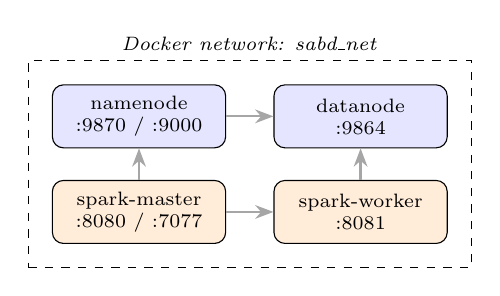
\begin{tikzpicture}[
    node distance=4mm and 6mm,
    box/.style={
        rectangle, draw, rounded corners, minimum height=8mm,
        minimum width=22mm, align=center, font=\scriptsize,
        fill=blue!10
    },
    sparkbox/.style={box, fill=orange!15},
    arrow/.style={-{Stealth}, thick, gray!70}
]
\node[box] (nn) {namenode\\\scriptsize :9870 / :9000};
\node[box, right=of nn] (dn) {datanode\\\scriptsize :9864};
\node[sparkbox, below=of nn] (sm) {spark-master\\\scriptsize :8080 / :7077};
\node[sparkbox, right=of sm] (sw) {spark-worker\\\scriptsize :8081};
\draw[arrow] (nn) -- (dn);
\draw[arrow] (sm) -- (sw);
\draw[arrow] (sm) -- (nn);
\draw[arrow] (sw) -- (dn);
\node[draw, dashed, fit=(nn) (dn) (sm) (sw),
      inner sep=3mm, label=above:{\scriptsize \emph{Docker network: sabd\_net}}] {};
\end{tikzpicture}

\column{0.45\textwidth}
\small
\textbf{HDFS layer} (storage)
\begin{itemize}\footnotesize
    \item \texttt{bde2020/hadoop-namenode}
    \item \texttt{bde2020/hadoop-datanode}
    \item Replication 1 (single-node teaching)
\end{itemize}

\textbf{Spark layer} (compute)
\begin{itemize}\footnotesize
    \item \texttt{bde2020/spark-master}
    \item \texttt{bde2020/spark-worker}
    \item Spark 3.3.0
\end{itemize}

\textbf{Orchestration}: Docker Compose,\\one YAML, reproducible.
\end{columns}

\vspace{0.5em}
\centering
\footnotesize\textbf{Bring it up:} \texttt{docker compose -f
docker/docker-compose.yml up -d}

\note{
The deployment is four Docker containers in a single private
network. Two for HDFS (namenode and datanode), two for Spark
(master and worker). Everything is described in a single
docker-compose YAML, so the cluster can be reproduced from
scratch with one command. I use bde2020 images because they
come pre-configured for HDFS and Spark to discover each other.
}
\end{frame}

% =============================================================
\begin{frame}{Code Organization}
Three layers mirror the runtime:

\begin{block}{Reusable helpers --- \texttt{utils.py}, \texttt{preprocessing.py}}
\begin{itemize}
    \item \texttt{utils.py}: timing context manager, list of relevant columns
    \item \texttt{preprocessing.py}: SparkSession construction, schema-aware loader
\end{itemize}
\end{block}

\begin{block}{One script per query}
\begin{itemize}
    \item \texttt{query1.py}, \texttt{query2.py}: pure query logic
    \item \texttt{plot\_q1.py}, \texttt{plot\_q2.py}: visualization (pandas + matplotlib)
    \item \texttt{benchmark.py}: harness that runs queries N times for stats
\end{itemize}
\end{block}

\begin{alertblock}{Migration local $\rightarrow$ HDFS was 1 line of code}
Only \texttt{preprocessing.py} had to read the Spark master URL from
an environment variable. Everything else is unchanged.
\end{alertblock}

\note{
The codebase is intentionally split into three layers. Utilities
that I use everywhere, the Spark setup which is shared between
both queries, and one script per concrete query. This
separation paid off when moving from local CSV to HDFS: I only
modified the preprocessing module. The query files themselves
did not change at all.
}
\end{frame}

% =============================================================
\section{Queries}
\begin{frame}{Query 1 --- Monthly stats for AA and DL}
\textbf{Goal}: for American Airlines and Delta, per month:
\begin{itemize}\small
    \item average / minimum / maximum \texttt{DEP\_DELAY} (non-cancelled flights only)
    \item cancellation rate (over all flights)
\end{itemize}

\begin{columns}[T]
\column{0.45\textwidth}
\textbf{Implementation key points}
\begin{itemize}\footnotesize
    \item Filter to \{AA, DL\}
    \item \texttt{cache()} the filtered DataFrame
    \item It feeds \textbf{two} aggregations:
    \begin{itemize}
        \item delay stats (non-cancelled subset)
        \item cancellation rate (all)
    \end{itemize}
    \item \texttt{join} on (month, airline)
    \item \texttt{coalesce(1)} for single CSV
\end{itemize}

\column{0.55\textwidth}
\centering
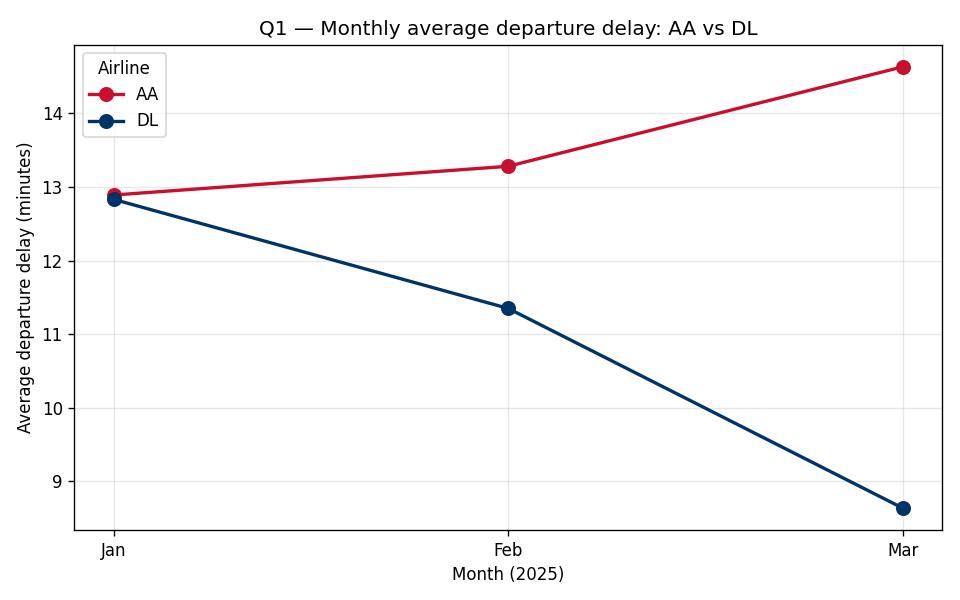
\includegraphics[width=\linewidth]{../plots/q1_avg_dep_delay.png}\\
\tiny Monthly avg departure delay (AA vs DL)
\end{columns}

\note{
Query 1 compares American Airlines and Delta on a monthly basis.
For non-cancelled flights it computes the average, minimum and
maximum departure delay. Separately, for ALL flights including
cancelled ones, it computes the cancellation rate. Because the
filtered DataFrame is used twice in two independent aggregations,
I cache it explicitly. Without caching, Spark would re-execute
the lineage from the CSV read on every action. The final
coalesce(1) gives me a single CSV file as the project expects.
}
\end{frame}

% =============================================================
\begin{frame}{Query 1 --- Results}
\begin{columns}[T]
\column{0.45\textwidth}
\centering
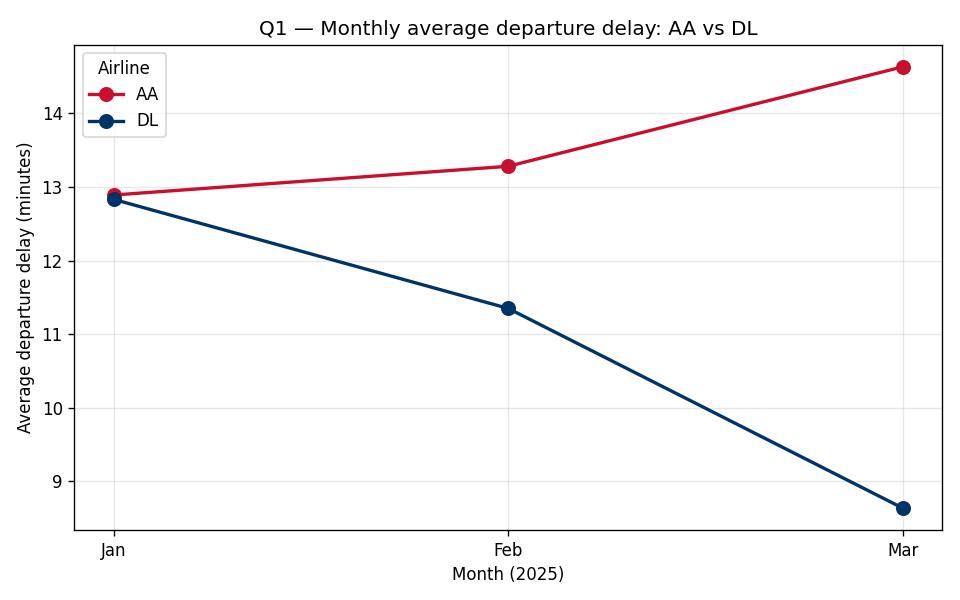
\includegraphics[width=\linewidth]{../plots/q1_avg_dep_delay.png}\\
\tiny Average departure delay

\column{0.55\textwidth}
\centering
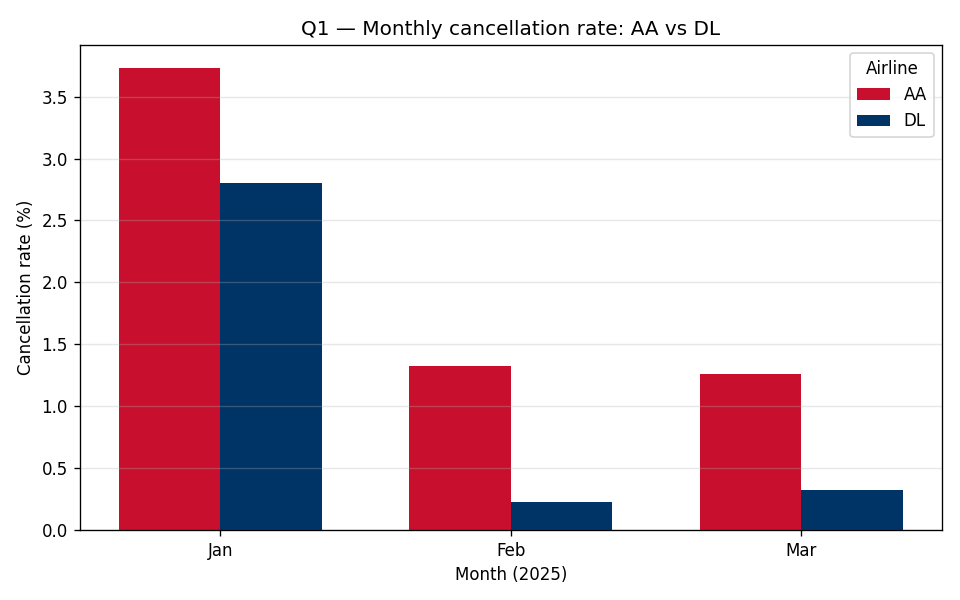
\includegraphics[width=\linewidth]{../plots/q1_cancellation_rate.png}\\
\tiny Cancellation rate
\end{columns}

\vspace{0.5em}
\small
\textbf{What we observe}:
\begin{itemize}\small
    \item Average delay is comparable between AA and DL ($\sim$8--15 min)
    \item Delta has a \textbf{much lower cancellation rate} (peak 2.8\% in Jan vs AA peak 3.7\%)
    \item January is the worst month for both (winter weather)
\end{itemize}

\note{
On the left, the monthly average departure delay. Both carriers
behave similarly. On the right, the cancellation rate: Delta
clearly outperforms American Airlines, especially in January.
The January peak in cancellations matches what you would
intuitively expect from winter storms in the United States.
}
\end{frame}

% =============================================================
\begin{frame}{Query 2 --- Top 10 by arrival delay}
\textbf{Goal}: rank carriers by mean \texttt{ARR\_DELAY}, considering
only carriers with at least 500 \emph{completed} flights, and break
down the contribution of the 5 delay causes.

\begin{columns}[T]
\column{0.45\textwidth}
\textbf{Implementation key points}
\begin{itemize}\footnotesize
    \item Filter: \texttt{CANCELLED=0 AND DIVERTED=0}
    \item NULL delay-cause columns $\rightarrow$ 0\\
          \scriptsize (BTS convention: filled only when ARR\_DELAY $\geq$ 15)
    \item Single \texttt{groupBy} with 7 aggregations in parallel
    \item Filter \texttt{num\_flights $\geq$ 500}
    \item \texttt{orderBy desc + limit(10)}
\end{itemize}

\column{0.55\textwidth}
\centering
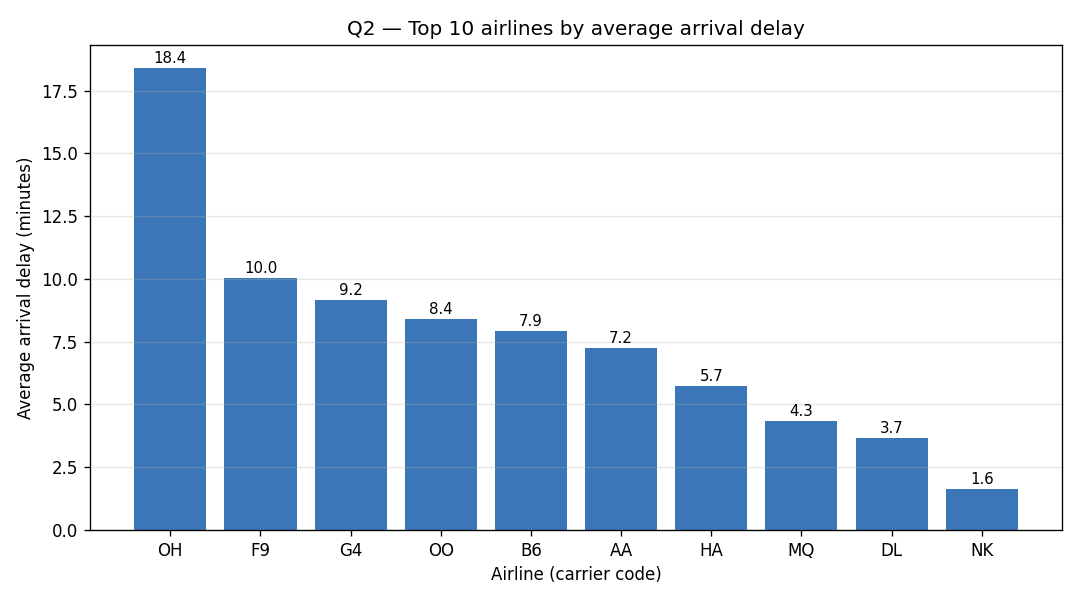
\includegraphics[width=\linewidth]{../plots/q2_top10_ranking.png}\\
\tiny Top 10 carriers ranked by mean arrival delay
\end{columns}

\note{
Query 2 ranks every carrier by average arrival delay, keeping
only the ones with at least 500 completed flights. The five
delay-cause columns are often NULL because the BTS only fills
them when the arrival delay exceeds 15 minutes. I treat NULL as
zero, meaning "this cause did not contribute". The alternative
of dropping NULLs would bias the average upwards because it
would keep only the delayed flights. I justified this choice
explicitly in the report.
}
\end{frame}

% =============================================================
\begin{frame}{Query 2 --- Cause breakdown}
\centering
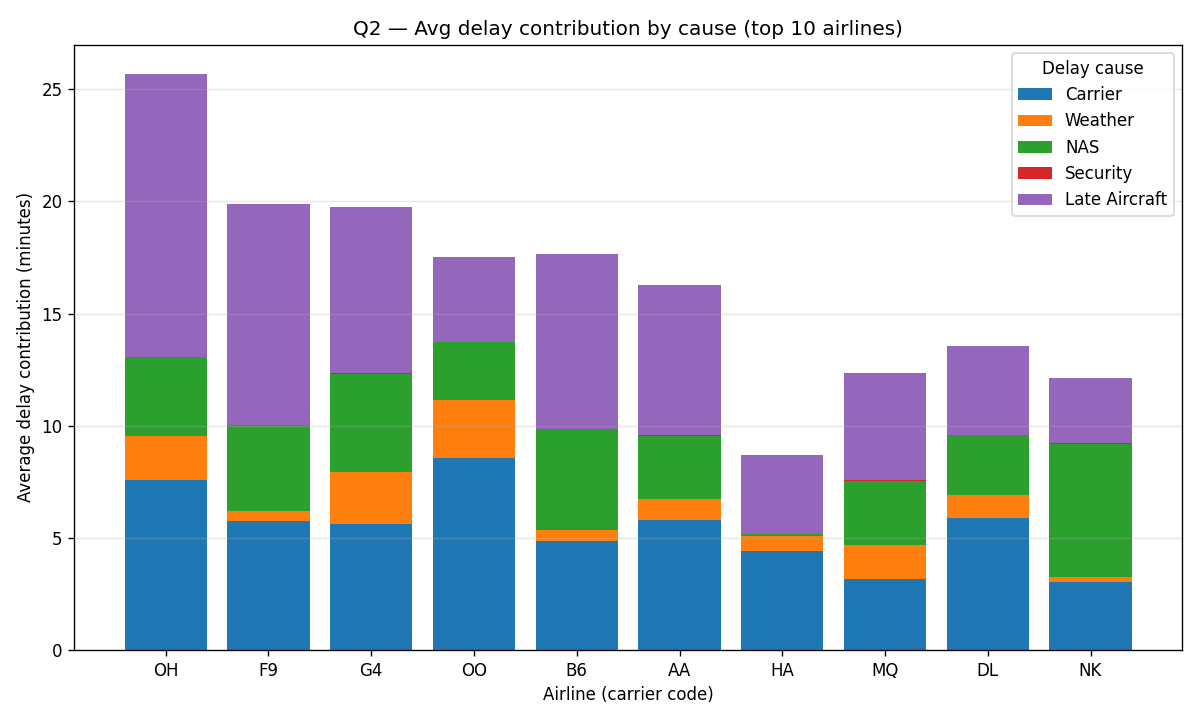
\includegraphics[width=0.7\linewidth]{../plots/q2_delay_causes.png}

\vspace{0.5em}
\small
\textbf{Dominant pattern}: \texttt{LATE\_AIRCRAFT\_DELAY} is the largest
contributor for the worst-performing carriers (OH, F9).\\
This is the \textbf{cascading effect}: one delay propagates downstream
through the day's flight rotation.

\note{
The stacked bar chart shows where the delay comes from for each
of the top 10 carriers. The dominant cause for the worst
performers is LATE_AIRCRAFT_DELAY, which is exactly the
domino effect: if your morning flight is late, every subsequent
flight using that aircraft will also be late. Weather and
security are minor contributors across the board.
}
\end{frame}

% =============================================================
\section{Key Implementation Decisions}
\begin{frame}{Four design decisions I would defend}
\begin{block}{1. Explicit schema (\texttt{StructType}) instead of \texttt{inferSchema}}
\texttt{inferSchema=true} would re-scan the entire CSV just to deduce
types. Explicit schema halves loading time and prevents silent type
mismatches.
\end{block}

\begin{block}{2. \texttt{cache()} only when the DataFrame is reused}
Q1 caches (used twice). Q2 does not (used once). Caching for the
sake of caching wastes memory and triggers an extra materialization.
\end{block}

\begin{block}{3. \texttt{shuffle.partitions = 8} (Spark default: 200)}
For 1.5\,M records on one machine, 200 partitions create scheduling
overhead with mostly-empty work units. Setting it to the CPU count
removes that overhead.
\end{block}

\begin{block}{4. \texttt{coalesce(1)} at output --- a trade-off}
Forces a final shuffle but produces \textbf{a single CSV per query} as
required by the spec. Removing it would save $\sim$2\,s but force the
user to concatenate eight part-files by hand.
\end{block}

\note{
These are the four decisions I am most likely to be asked about.
First: explicit schema, because inferSchema requires a second
pass over the data just to infer types. Second: caching is not
free, I only cache when I actually reuse the DataFrame. Third:
the default 200 shuffle partitions is way too many for our data
size on a single machine, eight matches the CPU count. Fourth:
coalesce(1) is a deliberate trade-off; it costs about two
seconds but it gives the user a single result file, which is
what the specification requires.
}
\end{frame}

% =============================================================
\section{Experimental Evaluation}
\begin{frame}{Benchmark methodology}
\textbf{Two configurations}:
\begin{itemize}
    \item \textbf{Local}: PySpark in venv, \texttt{master("local[*]")}, CSVs on disk
    \item \textbf{HDFS}: \texttt{spark-submit} on the dockerized cluster, CSVs in HDFS
\end{itemize}

\vspace{0.5em}
\textbf{Protocol per query, per configuration}: $6$ runs $=$ $1$ warm-up (discarded) $+$ $5$ measured

\vspace{0.5em}
\textbf{Why warm-up matters}: pilot run gave Q1 end-to-end of
\textbf{34.9\,s} on HDFS, against the steady-state \textbf{19.1\,s}.
The 16-second gap is JVM JIT compilation $+$ HDFS metadata caching.

\vspace{0.5em}
\textbf{Reported}: mean $\pm$ sample standard deviation across the 5
measured runs.

\note{
For each query and each configuration I run the benchmark six
times. I discard the first run as warmup, and report mean and
standard deviation across the remaining five. The warmup step is
critical: a pilot Q1 run on HDFS without warmup measured 35
seconds, while the steady state is 19. The 16-second difference
is JVM JIT compilation plus HDFS metadata caching warming up.
Without discarding that first iteration, every measured average
would be distorted.
}
\end{frame}

% =============================================================
\begin{frame}{Results --- Local vs HDFS}
\centering
\small
\begin{tabular}{l|rr|rr}
\toprule
& \multicolumn{2}{c|}{\textbf{Local}} & \multicolumn{2}{c}{\textbf{HDFS cluster}}\\
\textbf{Stage} & Q1 & Q2 & Q1 & Q2\\
\midrule
loading       & $3.96 \pm 0.61$ & $0.65 \pm 0.03$ & $15.18 \pm 0.71$ & $11.03 \pm 0.39$\\
preprocessing & $0.04 \pm 0.03$ & $0.10 \pm 0.01$ & $0.02 \pm 0.00$  & $0.14 \pm 0.01$\\
computation   & $0.21 \pm 0.04$ & $0.13 \pm 0.01$ & $0.23 \pm 0.05$  & $0.15 \pm 0.02$\\
output        & $1.69 \pm 0.26$ & $3.06 \pm 0.39$ & $3.65 \pm 0.29$  & $5.94 \pm 0.33$\\
\midrule
\textbf{end-to-end} & $\mathbf{5.89 \pm 0.86}$ & $\mathbf{3.94 \pm 0.41}$ & $\mathbf{19.09 \pm 0.83}$ & $\mathbf{17.27 \pm 0.57}$\\
\bottomrule
\end{tabular}

\vspace{1em}
\textbf{Overhead}: $\mathbf{3.2\times}$ for Q1, $\mathbf{4.4\times}$ for Q2 when moving to HDFS.

\note{
This is the headline table. Local times are around 4--6
seconds. HDFS times are around 17--19 seconds. The overhead is
roughly 3 to 4 times. The breakdown shows that the overhead is
concentrated in the loading and output stages, not in the
computation itself. That makes sense: the computation is
arithmetic that the CPU can do in milliseconds. What changes is
the I/O path.
}
\end{frame}

% =============================================================
\begin{frame}{Observations}
\begin{block}{1. Loading dominates the HDFS overhead}
$3.8\times$ slower for Q1, $17\times$ for Q2. Cost of:
namenode RPC, block-location lookup, streaming from datanode.
\end{block}

\begin{block}{2. Output is the second-largest HDFS cost (Q2: 5.9\,s)}
\texttt{coalesce(1)} shuffle + HDFS write path (block write,
metadata update, replication ack), amplified by container network.
\end{block}

\begin{block}{3. Computation is essentially unchanged}
Data volume is small relative to single-CPU capacity. The cluster
adds \emph{infrastructure} cost without adding \emph{compute} cost
at this scale.
\end{block}

\begin{block}{4. Steady-state $\neq$ first run}
Warm-up absorbs 5--15$\times$ the steady-state cost.
Mandatory in any honest benchmark.
\end{block}

\note{
Four take-aways. First, loading is the dominant HDFS cost,
because it triggers metadata round-trips to the namenode and
network transfers from the datanode. Second, output costs are
high because of the coalesce shuffle combined with HDFS
replication writes. Third, the actual computation time is the
same in both setups, because the dataset is small relative to
modern CPU capacity --- the cluster does not bring a speedup at
this scale, only overhead. Fourth, warm-up is mandatory; without
it the numbers are meaningless.
}
\end{frame}

% =============================================================
\section{Conclusions}
\begin{frame}{Conclusions}
\begin{block}{Delivered}
\begin{itemize}
    \item Containerized HDFS + Spark cluster (1 YAML)
    \item Q1 and Q2 implemented with the Spark DataFrame API
    \item 4 plots, 2 CSV deliverables, full benchmark suite
    \item Local vs HDFS comparison, end-to-end and per stage
\end{itemize}
\end{block}

\begin{block}{Main take-aways}
\begin{itemize}
    \item HDFS overhead is real, measurable and predictable at this scale
    \item Most performance wins come from \emph{decisions}, not from \emph{frameworks}\\
          (cache, schema, partitioning, coalesce)
    \item Reproducibility is achievable: one \texttt{compose up} brings
          the cluster, two scripts complete the pipeline
\end{itemize}
\end{block}

\note{
To wrap up: I delivered the containerized stack, the two queries
with all their visualizations, the CSV results, and the
benchmark suite. The main take-aways are that HDFS overhead is
real and measurable, that most performance wins come from
deliberate design decisions rather than from the framework
itself, and that reproducibility is achievable with one
docker-compose command and two shell scripts.
}
\end{frame}

% =============================================================
\begin{frame}
\centering
\Huge\textbf{Thank you}\\
\vspace{1em}
\Large Questions?\\
\vspace{2em}
\normalsize
\textit{Daniel Garoz \textendash{} SABD 2025/26 \textendash{} Project 1}

\note{
Thank you for your attention. I am happy to take any questions.
}
\end{frame}

\end{document}
